\clearpage
\appendix
\begin{center}{\large\bfseries Supplementary material}\\[2pt]\cad: Decision-Native Language Modeling of Single-Cell Gene Composition\end{center}
\suppressfloats[t]
\section{K-fold analysis on Norman}\label{app:kfold}
This analysis was run with the Qwen3.5-0.8B backbone (\cadf{}, the flat decoder of the population-level analysis) before the Gemma backbone was added.
\autoinput{auto/norman_kfold_table.tex}
\begin{figure}[t]
\centering
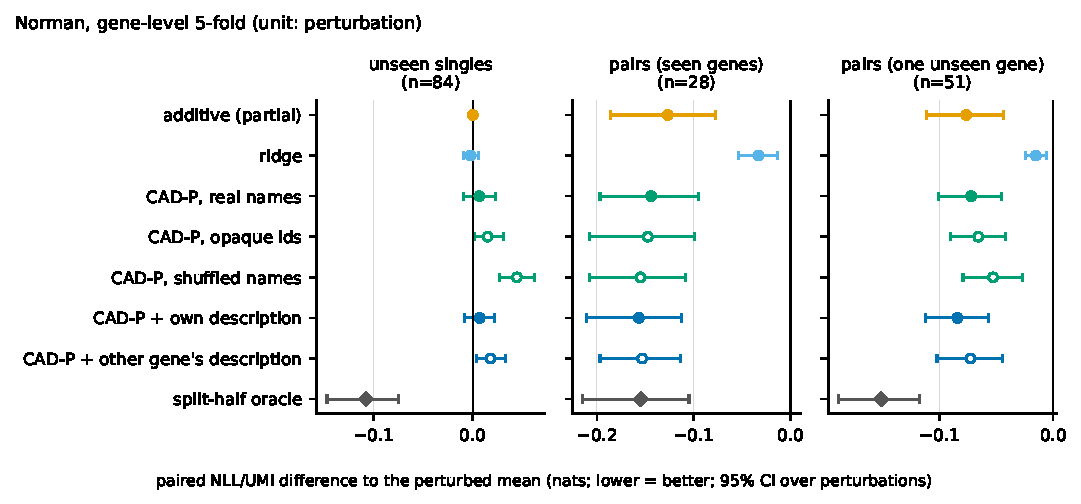
\includegraphics[width=\linewidth]{figs/fig_kfold_forest.pdf}
\caption{Gene-level 5-fold on Norman, population level: paired held-out NLL difference to the perturbed mean (bars: 95\% bootstrap over perturbations; hollow: identity or knowledge controls; diamond: split-half oracle).}
\label{fig:forest}
\end{figure}
Pooled over five gene-level folds, the flat decoder ties the partial-additive baseline on pairs of seen genes ($-0.017$, CI $-0.060$ to $+0.021$, $n=28$) and on pairs with one unseen gene ($+0.004$, CI $-0.014$ to $+0.022$, $n=51$), and it beats ridge.
The split-half oracle lies $0.108$ nats below the perturbed mean on unseen single genes, so headroom exists; descriptions and shuffled names do not help, and shuffled names are harmful ($+0.045$).
A one-parameter target-induction baseline, which raises the unseen target gene's frequency, is better than every learned decoder on the $75$ genes whose target is in the panel ($-0.013$, CI $-0.031$ to $-0.004$).
On the test split, \cadf{} (Qwen backbone) is $0.097$ better than the perturbed mean and ties additive ($-0.003$, CI $-0.031$ to $+0.019$).

\section{Training details}\label{app:train}
Table~\ref{tab:train} lists the training settings of the decision language models, and the paragraphs below it describe the scVI-based baselines.

\begin{table}[h]
\centering
\scriptsize
\begin{tabular}{@{}p{0.22\linewidth}p{0.74\linewidth}@{}}
\toprule
Setting & Value \\
\midrule
Optimizer, schedule & AdamW (weight decay $0$), one-cycle schedule with $5\%$ warm-up, gradient clipping at $1.0$ \\
Learning rates & $2\times10^{-4}$ (LoRA adapters), $10^{-3}$ (decision head, zero-initialized) \\
Batch size, budget & $16$; one epoch over $20{,}000$ training cells drawn at random ($1{,}250$ steps) \\
LoRA & rank $16$, $\alpha=16$, dropout $0$, all linear layers; rank $8$ and $64$ for the sensitivity run \\
Precision, attention & bf16; eager attention and gradient checkpointing for Gemma-2 \\
Output vocabulary & the $2048$ panel genes as classes; no new tokens, gene names are tokenized as plain text \\
Control-cell text & $48$ most abundant genes with $14$ log-mass levels; $200$ gene names for the rank variant \\
Seeds & test: Gemma and Qwen $0,1,2$; validation: Gemma $3407$ (default), $1$, $2$; Qwen $1,2$; variants of Appendix~\ref{app:protocol}: Qwen seed $0$ (the seed changes the sampled training cells and the sampler) \\
Negative-binomial head & inverse dispersion $\log\theta_g(c)=\beta_g+v_g^\top h$, initialized at $\theta=1$ and clipped to $[e^{-6},e^{8}]$; loss: negative-binomial NLL of the raw panel counts with mean $N_iq_g$, per UMI \\
Low-rank head & $k=16$ programs; amplitude $a(h)=\mathrm{softplus}(\cdot)$ initialized at $1$; encoder of the target cell: $\log(1+10^4x/N)\to256$ (GELU) $\to2k$; one reparameterized sample per cell; KL weight raised linearly from $0$ to $1$ over the first $30\%$ of steps \\
C2S-Gemma baseline & C2S-Scale-Gemma-2-2B, LoRA $r=16$ on all linear layers, lr $2\times10^{-4}$, one-cycle schedule, $20{,}000$ cells, one epoch, batch $16$ (micro-batches of $2$); control and target as top-200 rank sentences; loss on the response only; sampling with top-$k$ $50$, top-$p$ $0.95$, up to $1024$ new tokens \\
Evaluation & $M=50$ held-out control cells per perturbation, the same for every method (earlier runs: drawn separately per method); $300$ generated cells per unit \\
Hardware, time & one A100 40\,GB; run alone, Qwen takes $6$ to $8.5$ min and Gemma $9.5$ to $24$ min per run ($90$ to $100$ min with the 200-gene rank text; wall-clock was longer when jobs shared the GPU); Gemma peak memory $8.7$\,GB \\
\bottomrule
\end{tabular}
\caption{Training settings of the decision language models.}
\label{tab:train}
\end{table}

\paragraph{scVI and scANVI.}
Both are trained on training cells of the panel with a negative-binomial likelihood, $30$ latent dimensions and $60$ epochs (scANVI: $15$ further epochs with cell-type labels).
The frequency vector of a cell type is the mean decoder output over up to $3000$ training cells of that type.

\paragraph{scGen-style baseline.}
An scVI model is trained on all training cells.
The latent shift of a single gene is the mean latent state of its perturbed cells minus that of the control cells, the shift of a pair is the sum of the shifts of its known genes, and a perturbation with no known gene uses the mean shift of all training perturbations.
Each held-out control cell is encoded, shifted and decoded with library size one.

\section{Negative-binomial evaluation}\label{app:nb}
For a held-out cell $i$ of a unit with library size $s_i$ and model frequency $q$, the count of gene $g$ is scored as $\mathrm{NB}(x_{ig}\mid\mu=s_iq_g,\phi_g)$ with variance $\mu+\phi_g\mu^2$.
The dispersions $\phi_g$ come from a method-of-moments fit on library-normalized training counts with the within-unit variance pooled over units (median $\phi=26.5$ for PBMC and $9.0$ for Norman, clipped to $[10^{-3},10^2]$).
The score is the negative log-likelihood per UMI, which is on a different scale from the multinomial score because it includes the zeros, so only differences are compared (Table~\ref{tab:nb}).
It uses the pooled frequency of a unit, so it does not reward conditioning on a control cell.

\begin{table}[h]
\centering
\scriptsize
\begin{tabular}{llrr}
\toprule
Task & Model & $\Delta$NB [95\% CI] & $\Delta$multinomial \\
\midrule
PBMC (vs.\ cell-type mean) & global mean & $+0.302$ [$+0.252$, $+0.352$] & $+1.125$ \\
 & scVI & $+0.004$ [$+0.001$, $+0.007$] & $+0.005$ \\
 & scANVI & $+0.002$ [$+0.000$, $+0.005$] & $+0.004$ \\
 & \cadc{} (Gemma) & $+0.004$ [$+0.002$, $+0.006$] & $+0.017$ \\
 & \cadc{} (Qwen) & $+0.005$ [$+0.002$, $+0.009$] & $+0.030$ \\
\midrule
Norman (vs.\ perturbed mean) & additive & $-0.014$ [$-0.023$, $-0.004$] & $-0.094$ \\
 & ridge & $-0.008$ [$-0.010$, $-0.006$] & $-0.024$ \\
 & scGen-style & $-0.014$ [$-0.021$, $-0.008$] & $-0.085$ \\
 & \cadc{} (Gemma, no control) & $-0.021$ [$-0.027$, $-0.015$] & $-0.104$ \\
 & \cadc{} (Gemma, control) & $-0.017$ [$-0.023$, $-0.012$] & $-0.091$ \\
 & \cadc{} (Qwen, no control) & $-0.019$ [$-0.025$, $-0.013$] & $-0.092$ \\
 & \cadc{} (Qwen, control) & $-0.015$ [$-0.020$, $-0.010$] & $-0.078$ \\
\bottomrule
\end{tabular}
\caption{Negative-binomial and multinomial NLL per UMI relative to the reference (test split, seed 0; earlier runs, with control cells not matched across methods; negative favors the model; paired bootstrap over cell types or perturbations).}
\label{tab:nb}
\end{table}

On PBMC the negative-binomial score separates the decoders slightly more than the multinomial score does: \cadc{} is reliably, but marginally ($0.004$ nats), worse than the cell-type mean.
On Norman the ordering of the methods is the same as under the multinomial score.

\section{Worked examples: prompts and decoded distributions}\label{app:demo}
Figures~\ref{fig:demo} and~\ref{fig:demo2} show, for every use case, the exact prompt that the decision language model reads and the distribution it returns, next to the held-out ground truth.
The examples are not hand-picked.
In each case, the shown unit is the held-out cell type or perturbation whose paired NLL difference between \cad{} and the case's reference is the median over the units of that case, so half of the units look better and half look worse.
The cases are:
\begin{itemize}
\item conditional generation on unseen PBMC donors, against the cell-type mean;
\item perturbation response without a control cell, one example per stratum of the gene-level split (unseen single gene, pair with one unseen gene, pair of two seen genes), against the additive baseline;
\item perturbation response with a control cell, for a pair of two seen genes, once with the control cell both written as mass-level text in the prompt and used as the residual prior (the prompt shows a real serialized control cell), and once with the control cell used only as the residual prior;
\item zero-shot cell types (fold 0, so the median of its $4$ held-out types), against the mean of the nearest training type in the Cell Ontology.
\end{itemize}
The ground truth is the pooled frequency of all held-out real cells of the unit.
For a control-cell model the plotted distribution is the mean over the $M=50$ matched control cells, and the prompt shown is the one built from the first of them.
For perturbations, the right panel compares the log fold change over the held-out control mean on the unit's top-20 differentially expressed genes (largest $|t|$ of a Welch test between its real cells and the held-out control cells, computed on real cells only).
The selected units and the numbers quoted for them are:
\autoinput{figs/demo_outputs_text.tex}

\begin{figure}[p]
\centering
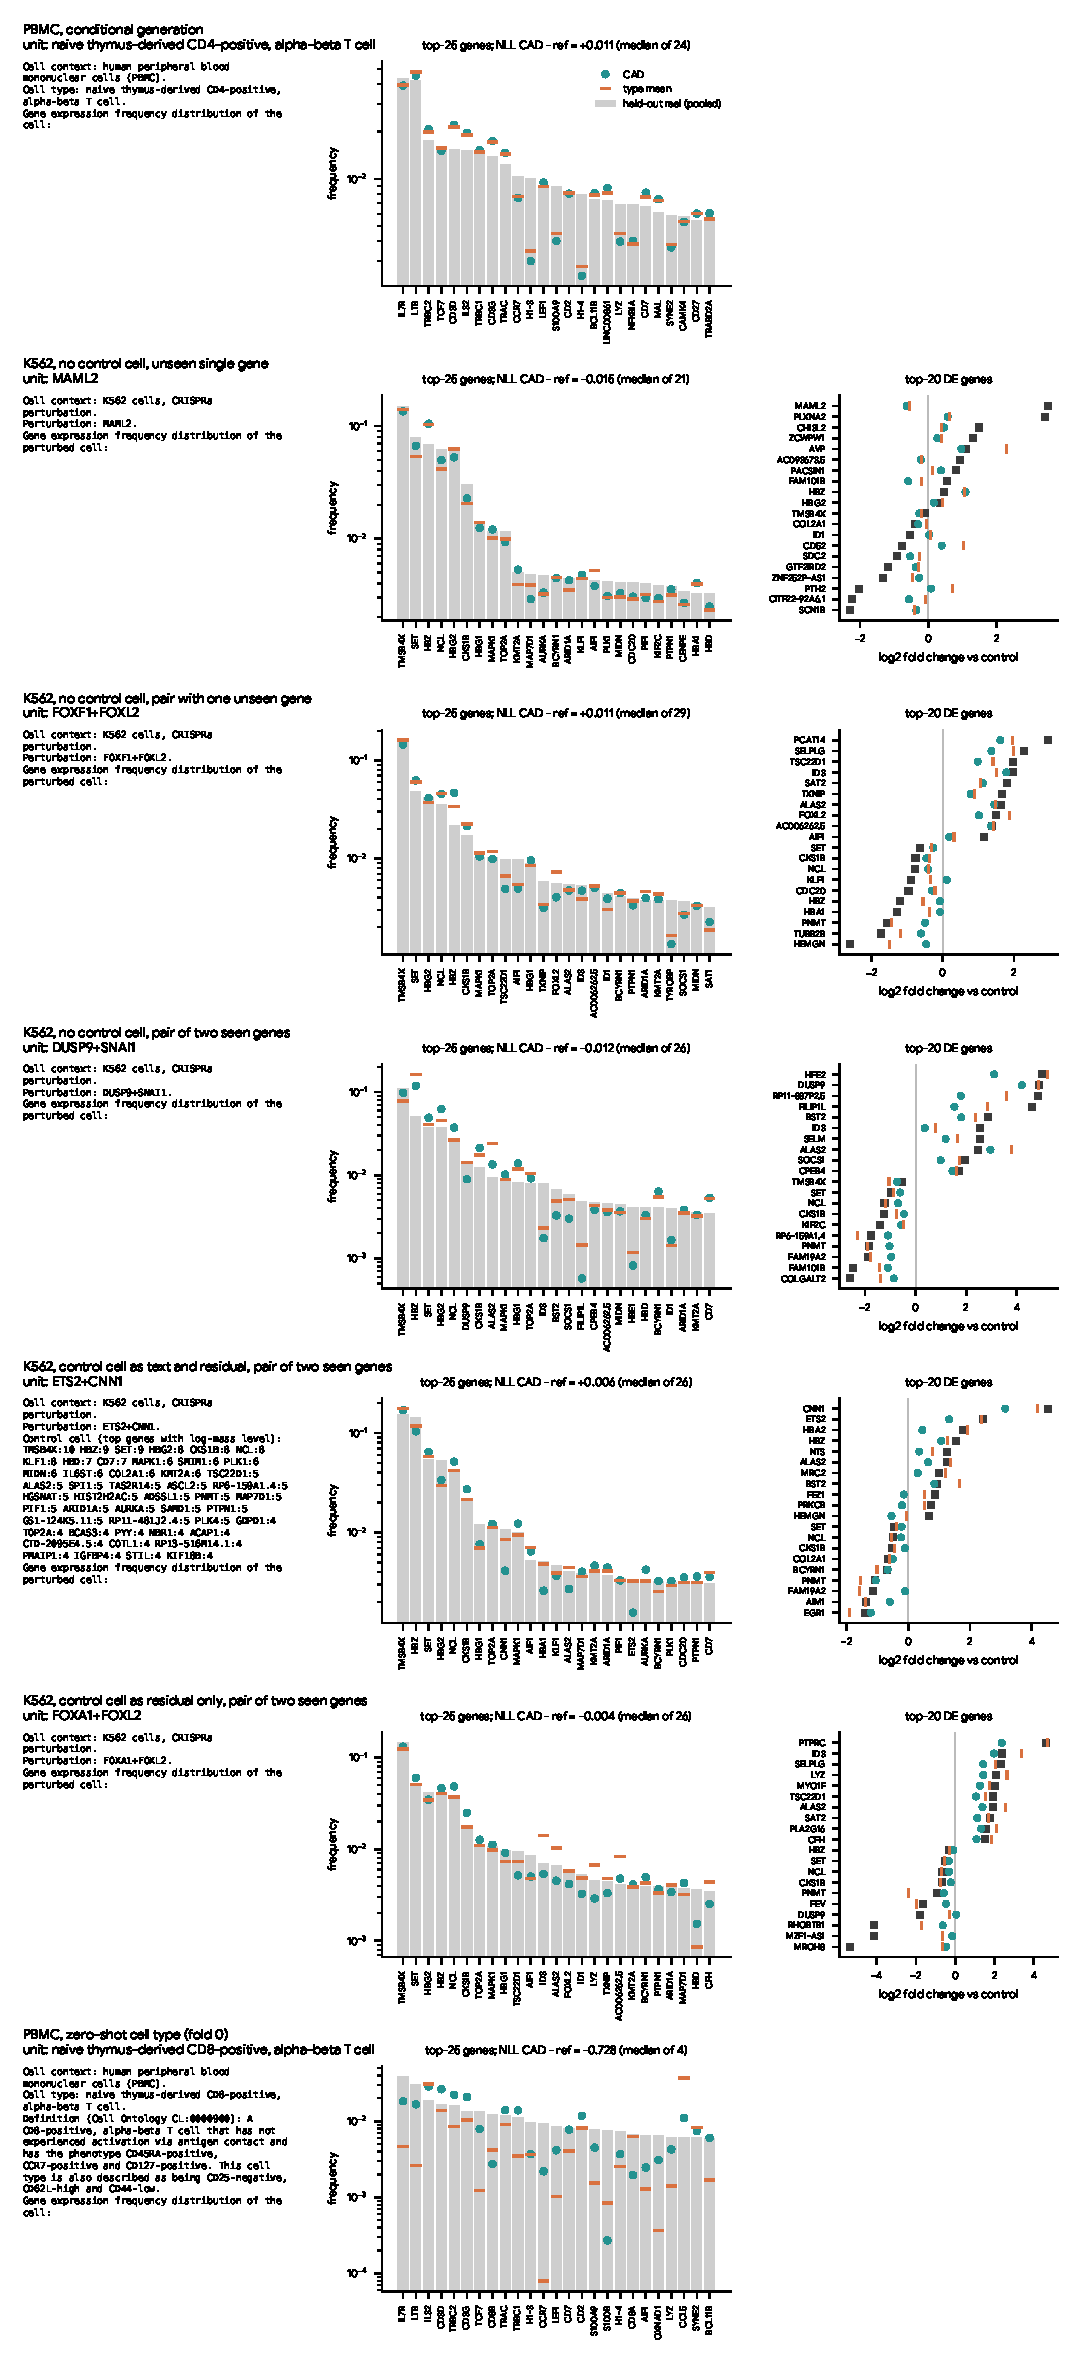
\includegraphics[width=0.94\linewidth,trim=0 484 0 0,clip]{figs/demo_outputs.pdf}
\caption{Prompts and decoded distributions, one median example per use case (test split). Left: the prompt given to \cad{}. Middle: frequency of the 25 genes with the highest ground-truth frequency (log scale) for the held-out real cells (grey bars), \cad{} (teal dots) and the reference (orange ticks). Right, perturbations only: log fold change over the held-out control mean on the unit's top-20 DE genes for real cells, \cad{} and the reference. Shown here: conditional generation and the three strata without a control cell; the remaining cases are in Figure~\ref{fig:demo2}.}
\label{fig:demo}
\end{figure}
\begin{figure}[p]
\centering
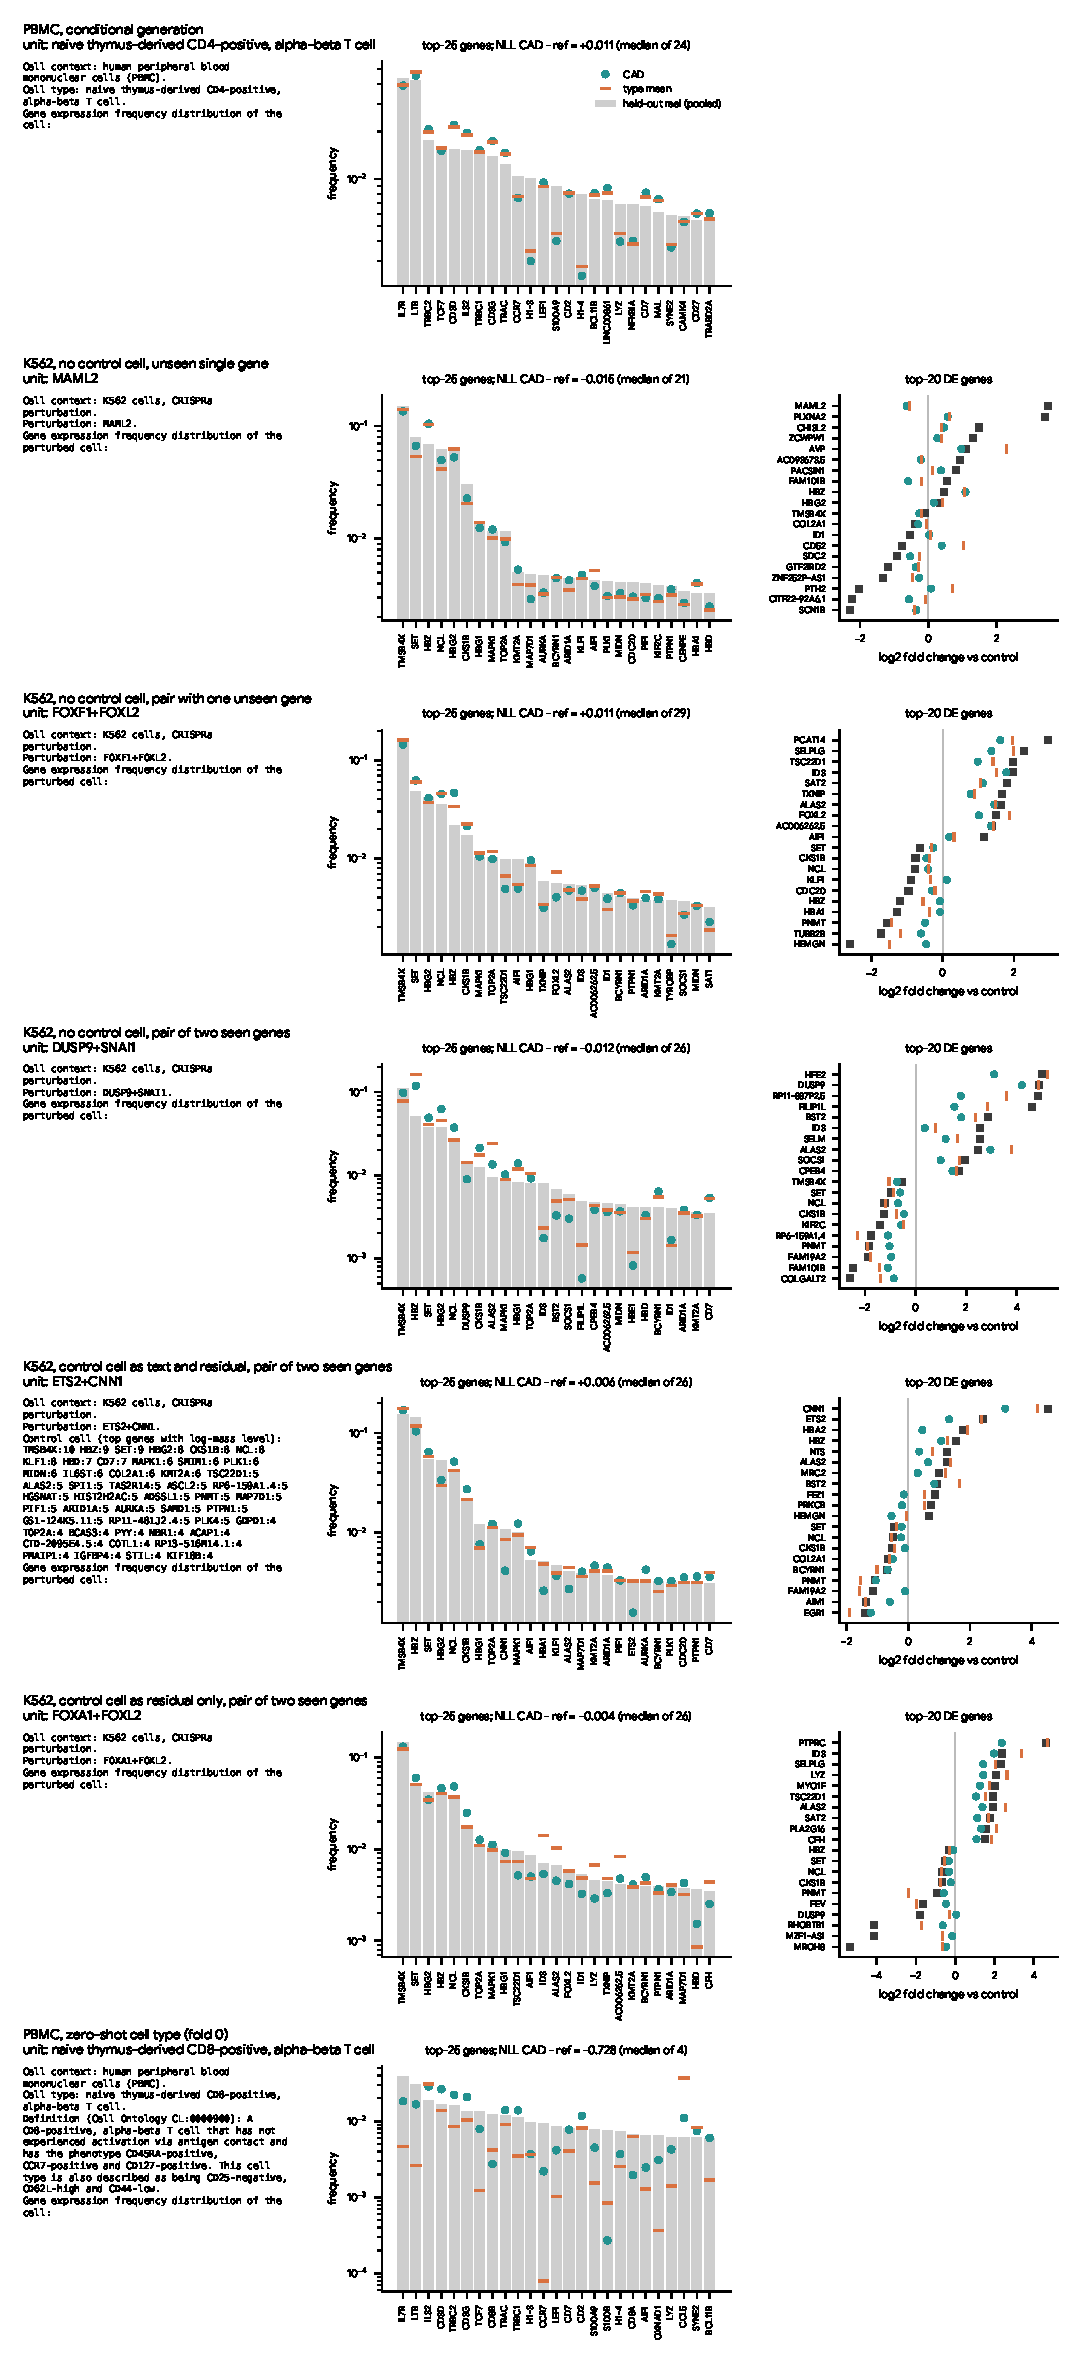
\includegraphics[width=0.94\linewidth,trim=0 0 0 650,clip]{figs/demo_outputs.pdf}
\caption{Prompts and decoded distributions (continued from Figure~\ref{fig:demo}): perturbation response with the control cell as text and residual, and as residual only, and zero-shot cell types.}
\label{fig:demo2}
\end{figure}

\section{Target transformations}\label{app:transform}
\autoinput{auto/pbmc_val_transform_table.tex}
Table~\ref{tab:pbmc_val_transform} (validation, $19$ cell types, Qwen3.5-0.8B backbone) shows that the transformation trades likelihood for sample quality on PBMC.
Frequency gives the best NLL, and smoothing is worse on every metric ($+0.172$ nats, 95\% CI $+0.144$ to $+0.196$; MMD $+0.074$).
Log1p and square-root targets are $+0.144$ and $+0.118$ nats worse in NLL, yet their MMD is lower ($-0.057$, CI $-0.107$ to $-0.016$, and $-0.057$, CI $-0.109$ to $-0.014$) with unchanged real-versus-generated AUC.
A flatter target moves mass to rarely expressed genes, which lowers the likelihood of raw counts while placing generated cells closer to real ones in PCA space.

For perturbation response the trade-off does not appear (Gemma backbone, test, $76$ perturbations; Appendix~\ref{app:val}).
Relative to the frequency target, log1p is $0.288$ nats worse in NLL (CI $+0.249$ to $+0.333$) and square root $0.250$ worse (CI $+0.219$ to $+0.282$), and both also have a higher MMD ($0.094$ and $0.087$ against $0.039$) and a higher real-versus-generated AUC ($0.875$ and $0.871$ against $0.811$).
We therefore keep frequency as the default, and we report the sample-quality advantage of flattened targets as specific to the conditional PBMC task in our experiments.


\section{UMAP views of generated cells}\label{app:umap}
\begin{figure}[t]
\centering
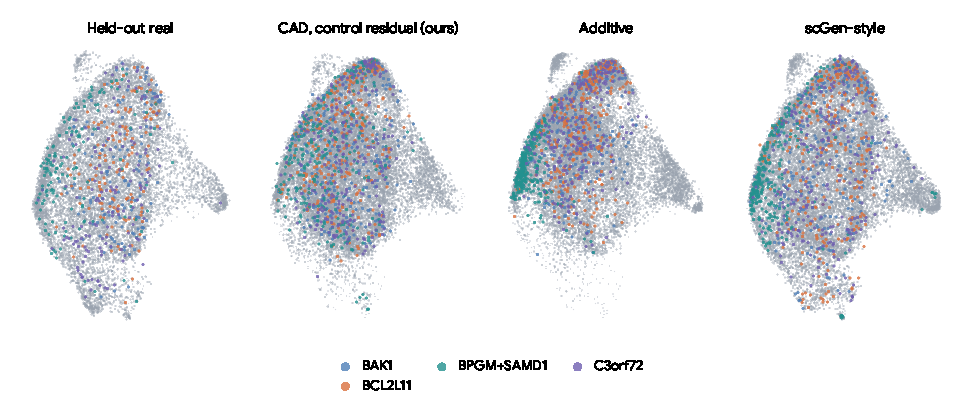
\includegraphics[width=\linewidth]{figs/umap_pert_rev2.pdf}
\caption{UMAP of held-out real perturbed K562 cells (test split) and of cells generated from the matched control cells by \cad{} with the control-cell residual (Gemma, seed 0), by the additive baseline and by the scGen-style latent shift, all drawn with the shared multinomial sampler. PCA and UMAP are fit on real cells only, and generated cells are projected. Colors: the four most frequent held-out perturbations; grey: the others.}
\label{fig:umap-pert}
\end{figure}
\begin{figure}[t]
\centering
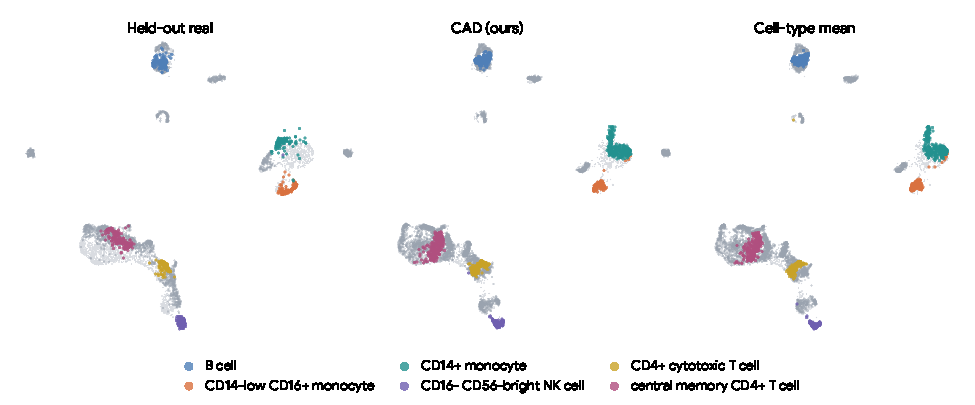
\includegraphics[width=\linewidth]{figs/umap_cond_rev2.pdf}
\caption{UMAP of held-out real PBMC cells (unseen donors, test split) and of cells generated by \cad{} (Gemma, seed 0) and by the cell-type mean with the same sampler. PCA and UMAP are fit on real cells only, and generated cells are projected. Colors: the six most frequent cell types; grey: the others.}
\label{fig:umap-cond}
\end{figure}

\section{Decision rules and the test-split record}\label{app:protocol}
Beyond the main configurations, every variant was first run on validation (Qwen3.5-0.8B backbone, seed~0, matched control cells, comparators re-run with the same control cells) and promoted to the test split only if, on validation, its paired 95\% interval against its comparator excluded zero in its favor on at least one metric fixed in advance, and no such metric was worse with an interval excluding zero; at most three new configurations were promoted. Promoted configurations were then run once per seed (0, 1, 2) on test with the Gemma backbone. The rules and decisions were written to the repository before the test runs.

\begin{table}[h]
\centering
\scriptsize
\setlength{\tabcolsep}{3pt}
\begin{tabular}{p{0.30\linewidth}p{0.22\linewidth}p{0.24\linewidth}p{0.16\linewidth}}
\toprule
Variant & Comparator & Primary metric(s) & Decision \\
\midrule
Control residual, no control text & control residual with mass text & per-cell NLL & beat comparator; test, 3 seeds \\
Control text, no residual & control residual with mass text & per-cell NLL & worse; test, 1 seed (ablation) \\
Contrast control text & control residual with mass text & per-cell NLL, MMD, $r_\Delta$ & promoted \\
Gene summaries in the prompt & other gene's summary; opaque ids & NLL, $r_\Delta$ on unseen singles & not promoted \\
UMI-weighted loss & same model, equal weights & NLL, $r_\Delta$, $r_{\mathrm{DE}}$ & not promoted \\
Negative-binomial head & softmax head & NLL, $r_\Delta$, $r_{\mathrm{DE}}$ & promoted (Norman only) \\
Low-rank head & softmax head & per-cell NLL, MMD, AUC & promoted (no control cell) \\
Zero-shot cell types & nearest Cell Ontology type & NLL & passed (gate G3) \\
C2S-Gemma mixing weight & --- & validation NLL & $0.9$ (grid maximum) \\
\bottomrule
\end{tabular}
\caption{Validation decisions taken before the test runs.}
\label{tab:decisions}
\end{table}

Four analyses were added after the test results had been seen, and are labeled as such where they appear: the $R^2$ of the rank reconstruction (Section~\ref{sec:repr}), the control-cell residual without a language model (Section~\ref{sec:residual}; a first version that divided by the pooled control frequency instead of the mean prior was not a fair analogue and was discarded), the name-overlap and Cell Ontology parent baselines for zero-shot types (Section~\ref{sec:condgen}), and the decoding-speed benchmark (Section~\ref{sec:backbone}). Each can only weaken our claims.

Deviations, all disclosed: a $128$-gene mass-level control text was not evaluated because it repeatedly ran out of GPU memory; three Qwen control-residual test runs ran out of memory during the test lanes and were re-run alone with the same configuration; and the zero-shot gate was applied on the $8$ types of folds 0 and 1 because three validation runs of folds 2--4 had run out of memory, which were then re-run (on all $19$ types the gate gives the same decision, $-0.476$ nats per UMI, CI $-0.971$ to $-0.123$).

\paragraph{Revision 3 (written before its new runs).} Two controls for the language model (a frozen backbone with an MLP head, and a decoder without a language model; Section~\ref{sec:lm}) were specified, with their comparators, metrics and decision rule, in \texttt{experiments/PREREGISTRATION\_rev3.md} before they were run. As controls rather than candidate improvements, they were run on validation (Qwen, seed 0) and then on test (Gemma, seeds 0--2) whatever their validation result. Four further analyses of saved outputs were added after the test results had been seen: the downstream and target metrics with the perturbed genes excluded and the additive-plus-target-induction baseline (Section~\ref{sec:pert}); the learned rank-to-frequency maps, including the re-decoding of the C2S-Gemma sentences (Section~\ref{sec:repr}); and the co-expression comparison (Appendix~\ref{app:coexpr}). They use no new training on test data. Without exclusion, the downstream code reproduces the earlier $r_{\mathrm{DE}}$ values exactly.

\section{Distributional heads}\label{app:heads}
\textbf{Negative-binomial head.} The head adds a per-gene inverse dispersion $\theta_g(c)$, $\log\theta_g(c)=\beta_g+v_g^\top h$, and is trained on the negative-binomial likelihood of the counts with mean $N_iq_g$, so high-mass genes no longer dominate the gradient. On the Norman test split (no control cell, against the softmax head) it raises $r_\Delta$ by $0.020$ (CI $0.012$ to $0.029$), and by $0.049$ on unseen single genes (CI $0.034$ to $0.067$), at a small cost in pooled multinomial NLL ($+0.015$, CI $+0.006$ to $+0.028$). On PBMC it did not help on validation and was not promoted.

\textbf{Low-rank logistic-normal head.} The logits become $z=Wh+\log b+U\,\mathrm{diag}(a(h))\,\epsilon$ with $\epsilon\sim\mathcal N(0,I_{16})$, so $q(c,z)$ varies from cell to cell along $16$ learned gene programs; training uses a variational bound with an encoder of the target cell, and generation draws $\epsilon$ from the prior. Without a control cell it lowers the cell NLL by $0.089$ (CI $0.080$ to $0.098$) on Norman, reaching the scGen-style model ($-0.009$, CI $-0.019$ to $+0.002$), and on PBMC from $5.623$ to $5.552$. The pooled NLL of the mean over draws is worse ($+0.062$, CI $+0.040$ to $+0.087$) and $r_\Delta$ lower ($-0.067$). The cell NLL is estimated from $50$ (Norman) or $300$ (PBMC) prior draws; this log-mean-exp estimator is biased upwards.

\section{Co-expression of generated cells}\label{app:coexpr}
\autoinput{auto_rev3/tab_coexpr.tex}
For each test perturbation with at least $100$ real cells, on the $100$ panel genes with the largest variance of log-normalized expression in training cells, we compared the gene--gene Pearson correlations across real cells with those across the method's generated cells (multinomial sampler), and the total variance and the share of variance on the first principal component (Table~\ref{tab:coexpr}; post hoc). With a median of about $216$ panel UMIs per cell, correlations are dominated by counting noise, and every generator is within $0.005$ of the others in correlation error. Resampling real cells of training perturbations is further from the held-out cells ($0.093$), so the generated cells reproduce perturbation-specific co-variation at least as well as real cells of other conditions. The low-rank head and the scGen-style shift, which model variation between cells explicitly, are slightly closer than the flat decoders, and the additive baseline under-disperses (variance ratio $0.94$).

\section{Additional tables}\label{app:val}
\autoinput{auto_rev3/tab_norman_full.tex}
The tables in this section and in Appendix~\ref{app:transform} come from the earlier runs, in which the control cells were drawn separately for each method; the main-text tables use matched control cells.
Table~\ref{tab:norman_test_transform} (test) compares the target transformations for perturbation response with the Gemma backbone, and Table~\ref{tab:norman_test_rank_vs_mass} (test) compares the two control-cell formats.
Tables~\ref{tab:val_cond} and~\ref{tab:val_pert} repeat the comparison with the other generators on the validation split, on which all decisions were made; Table~\ref{tab:val_pert_lora} shows the LoRA-rank sensitivity on Norman (validation).
\autoinput{auto_test/norman_test_transform_table.tex}
\autoinput{auto_test/norman_test_rank_vs_mass_table.tex}
\autoinput{auto_rev/val_cond_table.tex}
\autoinput{auto_rev/val_pert_table.tex}
\autoinput{auto_test/val_pert_lora_table.tex}

\section{Proofs}\label{app:proofs}
\textbf{Observation~\ref{prop:repr}.} (i) $x=Np$ recovers the counts from $(N,p)$, and $(N,p)$ is a function of $x$. Under $\mathrm{Mult}(N,q)$, $\log P(x)=\log\frac{N!}{\prod_gx_g!}+\sum_gx_g\log q_g=\text{const}+N\sum_gp_g\log q_g$, which by Gibbs' inequality is maximized over $q\in\Delta$ at $q=p$. (ii) For any $x$ with at least two distinct nonzero counts, $x$ and $2x$ have the same ordering and hence the same sentence, and so do $x$ and any count vector obtained by a strictly increasing change of the counts. (iii) $x$ and $2x$ have the same binarization. For $f(t)=\log(1+t)$ or $f(t)=\sqrt t$, the renormalized vector is $p'_g=f(x_g)/\sum_hf(x_h)$, and $p'=p$ requires $f(x_g)/x_g$ to be equal for all genes with $x_g>0$; because $f(t)/t$ is strictly decreasing for $t>0$, this holds only when all nonzero counts are equal.

Throughout, $\Delta$ is the simplex over the $G$ panel genes and modules $S_1,\dots,S_M$ partition the genes; P1, P3 and P4 concern the hierarchical head of Appendix~\ref{app:tree}, and P2 concerns the NLL used throughout.
\begin{description}
\item[P1 (normalization and exact factorization).] For any $q^{\mathrm{root}}\in\Delta^{M}$ and $q^{m}\in\Delta^{|S_m|}$, $q(g)=q^{\mathrm{root}}(m(g))\,q^{m(g)}(g)$ lies in $\Delta$, and for counts $X$ with module totals $n_m$,
\[-\sum_gX_g\log q(g)=-\sum_mn_m\log q^{\mathrm{root}}(m)-\sum_m\sum_{g\in S_m}X_g\log q^m(g).\]
Every $q$ in the interior of $\Delta$ factors uniquely this way, so the hierarchical head is a \emph{re-parametrization} of the flat head: it changes what the network must output, not the family of distributions it can represent.
\item[P2 (the metric is proper).] If the counts $X$ of a perturbation's cells satisfy $\mathbb{E}[X_g/\sum_hX_h]=\pi_g$ given the total, the expected NLL per UMI of $q$ is $H(\pi)+\mathrm{KL}(\pi\,\|\,q)$ and is uniquely minimized at $q=\pi$. Differences in expected NLL between two decoders therefore equal differences in $\mathrm{KL}(\pi\|q)$.
\item[P3 (tilt identity and its population minimizer).] For $f,\tilde p$ in the interior of $\Delta$, $q_g\propto f_gt_g$ equals $\tilde p_g$ exactly. If a context is paired with bags $b$ having tilts $t_b$, the minimizer of the expected soft cross-entropy is $\mathbb{E}[t_b]$, so the implied decoder is $q_g\propto\mathbb{E}_b[\tilde p_{b,g}/Z_b]$: a $1/Z_b$-weighted average of bag frequencies, which equals the plain average whenever $Z_b$ is constant within a context. The target is the shrunk $\tilde p$, so $\lVert\tilde p-p\rVert_1\le\tfrac{\lambda}{n+\lambda}\lVert f-p\rVert_1\le2\tfrac{\lambda}{n+\lambda}$ ($\approx1\%$ for $n\approx2\!\times\!10^5$ UMIs per bag).
\item[P4 (sampled-leaf loss).] Let $T_m=\sum_{g\in S_m}t_g$. With modules $A=(m_1,\dots,m_R)$ drawn i.i.d.\ from $T$, $\mathrm{CE}(T,r^{\mathrm{root}})+\mathbb{E}\big[\tfrac1R\sum_{r}\mathrm{CE}(t|_{m_r},r^{m_r})\big]=\mathrm{CE}(t,r)$, the full tree cross-entropy. \emph{Our implementation samples without replacement and the trainer averages questions with equal weight, so its record loss is a weighted surrogate} ($1/(R{+}1)$ per question), not this unbiased estimator; the two share their minimizer only when every conditional is exactly representable (the well-specified regime).
\end{description}
\textbf{P1.} $\sum_gq(g)=\sum_mq^{\mathrm{root}}(m)\sum_{g\in S_m}q^m(g)=\sum_mq^{\mathrm{root}}(m)=1$ and every factor is nonnegative. The loss identity follows from $\log q(g)=\log q^{\mathrm{root}}(m(g))+\log q^{m(g)}(g)$ and $\sum_{g\in S_m}X_g=n_m$. Conversely, for $q$ in the interior set $q^{\mathrm{root}}(m)=\sum_{g\in S_m}q(g)$ and $q^m(g)=q(g)/q^{\mathrm{root}}(m)$; these are the only factors that reproduce $q$ because $q^{\mathrm{root}}(m)=\sum_{g\in S_m}q(g)$ is forced by summing.

\textbf{P2.} Conditional on the total $N$, $\mathbb{E}[-\sum_gX_g\log q_g/N]=-\sum_g\pi_g\log q_g=H(\pi)+\mathrm{KL}(\pi\|q)$, and $\mathrm{KL}\ge0$ with equality if and only if $q=\pi$ (Gibbs' inequality). Two decoders therefore differ in expected NLL by $\mathrm{KL}(\pi\|q_A)-\mathrm{KL}(\pi\|q_B)$. Per-UMI scoring weights each perturbation's cells by their UMIs; the paired bootstrap treats the perturbation as the unit.

\textbf{P3.} $f_gt_g=\tilde p_g/Z$, so $\sum_hf_ht_h=1/Z$ and $f_gt_g/\sum_hf_ht_h=\tilde p_g$. For targets $t_b$ drawn with context $c$, \[\mathbb{E}_b[\mathrm{CE}(t_b,r)]=H(\mathbb{E}t_b)+\mathrm{KL}(\mathbb{E}t_b\|r)+\text{const}\] is minimized by $r=\mathbb{E}[t_b]$, so $q_g\propto f_g\mathbb{E}[t_{b,g}]=\mathbb{E}[\tilde p_{b,g}/Z_b]$, a $1/Z_b$-weighted mean of $\tilde p_b$. With $\tilde p=(1-w)p+wf$ and $w=\lambda/(n+\lambda)$, $\lVert\tilde p-p\rVert_1=w\lVert f-p\rVert_1\le2w$.

\textbf{P4.} The chain rule gives $\mathrm{CE}(t,r)=\mathrm{CE}(T,r^{\mathrm{root}})+\sum_mT_m\,\mathrm{CE}(t|_m,r^m)$ with $t|_m=t_{S_m}/T_m$. For $m_1,\dots,m_R$ i.i.d.\ from $T$, $\mathbb{E}[\mathrm{CE}(t|_{m_r},r^{m_r})]=\sum_mT_m\mathrm{CE}(t|_m,r^m)$ for each $r$, which gives the claim. Sampling without replacement changes the inclusion probabilities away from $T_m$, and averaging over the $R{+}1$ answered questions gives each question weight $1/(R{+}1)$ instead of $(1,\tfrac1R,\dots,\tfrac1R)$; if every conditional is representable, each term is minimized at the true conditional and the minimizer is unchanged.
\section{Hierarchical head ablation}\label{app:tree}
The hierarchical variant (\cadn{}/\cadr{}) answers one 64-option module question and four 32-option gene questions through the Unsloth decision head, trained on a \emph{tilt} target (the ratio of the perturbed to the control frequency, renormalized, with the control prior $f$ multiplied back at generation). On the corrected Norman split, trained on absolute frequencies it is $+0.161$ [$+0.150$, $+0.174$] nats worse than the perturbed mean (control-state NLL $5.490$ against $5.295$ for the control frequencies); the tilt repairs the fit (control $5.300$; tilt minus no-tilt $-0.138$ [$-0.157$, $-0.119$]) but the tilted head remains $+0.023$ [$+0.009$, $+0.038$] worse than the perturbed mean and $0.100$ nats worse than the flat head. The biological partition beats a random one by $0.019$ ($[-0.035,-0.002]$). We therefore use the flat head in the main text.
\end{document}
